\chapter{Opti-CAM: Optimizing saliency maps for interpretability}
\chaptertoc{}
%--------------------------------------------------------------------------------------------------
\label{ch:opticam}
% Introduction, to move to a more verbatum approach
\section{Introduction}
\label{sec:oc_intro}
\noindent Within existing attribution approaches for interpretable saliency map generation, the CAM  
\autocite{zhou2016learning} based family of methods takes special interest given its reliance of
existing  information and properties of a given model to generate explanations. In particular, 
following \autoref{eq:sal}, modifying computation of the weighting coefficient 
$w_k^c$ results in a different attribution being generated. Moreover, this computation can be 
altered, for instance by relying on information found while performing the backward pass 
(\cite{selvaraju2017grad}, \cite{chattopadhay2018grad}, \cite{axiombased}, 
\cite{smilkov2017smoothgrad}) and the forward pass \autocite{wang2020score} of the model during 
inference. Nevertheless, we observe that among existing weighting coefficient computation 
proposals, none has been directed at maximizing the predicted probability of the generated 
 saliency maps.\\

\noindent Complementary to CAM methods, we observe that within attribution methods based on 
extremal perturbations \autocite{fong2019understanding} or IBA \autocite{schulz2020restricting}, 
their class scores are optimized via gradient descent. In this regard, it can 
be stated that these masks then become variables within input-feature space, and the aforementioned 
scores then become a function of said masking. However, it is important to point that optimizing 
these masks ultimately becomes an expensive process, as several constraints are needed 
to be taken into consideration to further control the masking area.\\

\noindent Drawing inspiration from the aforementioned observations, we set ourselves to design 
\emph{Opti-CAM}, an attribution method that generates saliency maps with enhanced interpretability. 
In particular, we hypothesize that the weighting coefficient $w_k^c$ can be optimized to attain 
this task; moreover, we also suggest that should the predicted probability of the attribution map 
is optimized, we can gain insight within the regions of the image that appear to be the most 
important for the classifier. We define our approach in \autoref{sec:oc_def}\\

\noindent In addition to the proposal of an attribution method in this chapter, we
design a complementary interpretability evaluation metric of saliency maps. In particular, 
based on the remarks found in Fake-CAM \autocite{poppi2021revisiting}, we observe that 
existing metrics such as \gls{ad} (\ref{eq:ad}) and \gls{ai} (\ref{eq:ai}) can be manipulated. As a 
result of this, we argue that a complementary criterion is missing regarding \textit{Objective 
Evaluation for Object Recognition}. In \autoref{sec:av_gain} we define this novel measurement 
under the name \gls{ag}. To support our approach, we demonstrate our generated saliency maps in 
\autoref{sec:oc_qual}, and we evaluate them in \autoref{sec:oc_quant}.\\

\noindent To sum up, with the observations previously mentioned, in this chapter we propose a CAM 
variant that generates saliency maps by optimizing the weighting coefficient $w_k^c$, while also 
introducing a novel metric to complement the existing evaluation of attribution methods.\\

\section{Preliminaries}
\label{sec:oc_prelim}

\paragraph{Notation}
\label{sec:oc_notation}

Consider a classifier network $f: \cX \to \real^C$ that maps an input image $\mathbf{u} \in \cX$ to a 
logit vector $\vy = f(\mathbf{u}) \in \real^C$, where $\cX$ is the image space and $C$ is the number 
of classes. We denote by $y_c = f(\mathbf{u})_c$ the predicted logit and by $p_c = \softmax(\vy)_c 
\defn e^{y_c} / \sum_j e^{y_j}$ the predicted probability for class $c$. For layer $\ell$ 
with $K_\ell$ channels, we denote by $A^k_\ell = f^k_\ell(\mathbf{u}) \in \real^{h_\ell \times w_\ell}$ 
the feature map for channel $k \in \{1,\dots,K_\ell\}$, with spatial resolution $h_\ell \times 
w_\ell$. Because of $\relu$ non-linearities, we assume that feature maps are non-negative. 
Similarly, we denote by $S_\ell \in \real^{h_\ell \times w_\ell}$ a 2D saliency map.

%--------------------------------------------------------------------------------------------------

\paragraph{Background: CAM-based saliency maps}
\label{sec:oc_back}

Given a layer $\ell$ and a class of interest $c$, we consider saliency maps given by the general 
formula
\begin{equation}
	S^c_\ell(\mathbf{u}) \defn h \left( \sum_k w^c_k A^k_\ell \right),
\label{eq:sal}
\end{equation}
where $w^c_k$ are weights defining a linear combination over channels and $h$ is an activation 
function. CAM \parencite{zhou2016learning} is defined for the last layer $L$ only with $h$ being the 
identity mapping and $w^c_k$ being the classifier weight connecting the $k$-th channel with 
class $c$. Grad-CAM \parencite{selvaraju2017grad} is defined for any layer $\ell$ with $h = \relu$ and 
weights
\begin{equation}
	w^c_k \defn \gap \left( \pder{y_c}{A^k_\ell} \right),
\label{eq:gcam}
\end{equation}
where $\gap$ is global average pooling.
% and $\softmax(\vy)_c = e^{y_c} / \sum_j e^{y_j}$ is the predicted probability of class $c$.
The motivation for $\relu$ is that we are only interested in features that have a positive effect 
on the class of interest, \ie pixels whose intensity should be increased in order to increase $y_c$.

Score-CAM \parencite{wang2020score} is also defined for any layer $\ell$ with $h = \relu$ and weights 
$w^c_k \defn \softmax(\mathbf{u}^c)_k$.  Softmax normalization considers positive channel contributions 
only and attends to few feature maps.
%that \alert{produce less highlighted areas in the saliency map}. \iavr{Last part unclear.}
Here, vector $\mathbf{u}^c \in \real^{K_\ell}$ measures the increase in confidence for class $c$ that 
compares a known baseline image $\mathbf{u}_b$ with the input image $\mathbf{u}$ masked according to feature 
map $A^k_\ell$, for all channels $k$:

\begin{equation}
	u^c_k \defn f(\mathbf{u} \odot n(\operatorname{up}( A^k_\ell )))_c - f(\mathbf{u}_b)_c,
\label{eq:s-cam}
\end{equation}

where $\odot$ is the Hadamard product. For this to work, the feature map $A^k_\ell$ is adapted
 to $\mathbf{u}$ first$:\operatorname{up}$ denotes upsampling to the spatial resolution of $\mathbf{u}$ and

\begin{equation}
	n(A) \defn \frac{A - \min A}{\max A - \min A}
\label{eq:norm}
\end{equation}

is a normalization of matrix $A$ into $[0,1]$. While Score-CAM does not need gradients, 
it requires as many forward passes through the network as the number of channels in the chosen layer,
 which is computationally expensive.

%--------------------------------------------------------------------------------------------------

\paragraph{Motivation}
\label{sec:motiv}

\iavr{Score-CAM considers each feature map as a mask in isolation. How about linear combinations?} 
Given a vector $\vw \in \real^{K_\ell}$ with $w_k$ its $k$-th element, let
\begin{equation}
	F(\vw) \defn f \left( \mathbf{u} \odot n \left( \operatorname{up} \left(
		\displaystyle\sum_k w_k A^k_\ell
	\right) \right) \right)_c.
\label{eq:s-obj}
\end{equation}
\ronan{If we assume that $\mathbf{u}_b = \vzero$ in~\eq{s-cam} and define $n(\vzero) \defn \vzero$ 
in~\eq{norm}, then we can rewrite the right-hand side of~\eq{s-cam} as
\begin{equation}
	\frac{F(\vw_0 + \delta \ve_k) - F(\vw_0)}{\delta},
\label{eq:s-cam2}
\end{equation}
where $\vw_0 = \vzero$, $\delta = 1$ and $\ve_k$ is the $k$-th standard basis vector of 
$\real^{K_\ell}$. This resembles the numerical approximation of the derivative $\pder{F}{w_k}(\vw_0)$,
 except that $\delta$ is not small as usual. One could compute derivatives efficiently by 
 standard backpropagation instead. It is then possible to iteratively optimize $F$ with respect
  to $\vw$, starting at any $\vw_0$.}

\iavr{As an alternative, consider masking-based methods relying on optimization in the input space, 
like \emph{meaningful perturbations} (MP) \parencite{fong2017interpretable} or 
\emph{extremal perturbations} \parencite{fong2019understanding}. In general, optimization takes the form
\begin{equation}
	S^c(\mathbf{u}) \defn \arg\max_{\vm \in \cM} f(\mathbf{u} \odot n(\operatorname{up}(\vm)))_c + \lambda R(\vm).
\label{eq:mask}
\end{equation}
Here, a mask $\vm$ is directly optimized and does not rely on feature maps, hence the saliency 
map $S^x(\mathbf{u})$ is not connected to any layer $\ell$. The mask is at the same or lower resolution 
than the input image. In the latter case, upsampling is still necessary.

In this approach, one indeed computes derivatives by backpropagation and indeed iteratively 
optimizes $\vm$. However, because $\vm$ is high-dimensional, there are constraints expressed by 
$\vm \in \cM$, \eg $\vm$ has a certain norm, and regularizers like $R(\vm)$, \eg $\vm$ is smooth in a 
certain way. This makes optimization harder or more expensive and introduces more hyperparameters 
like $\lambda$. One could simply constrain $\vm$ to lie in the linear span of $\{A_\ell^k\}_{k=1}
^{K_\ell}$ instead, like all CAM-based methods.}
\section{Opti-CAM}
As motivated by \textbf{motif}, we obtain a saliency map as a convex combination of feature maps
 by optimizing a given objective function with respect to the weights.
In particular, following \autocite{wang2020score}, we use channel weights $w_k \defn \softmax(
	\mathbf{u})_k$, where $\mathbf{u} \in \real^{K_\ell}$ is a variable.
We then consider saliency map $S_\ell$ in layer $\ell$ as a function of both the input image $\vx$ 
and variable $\mathbf{u}$:

\begin{equation}
    S_\ell(\vx; \mathbf{u}) \defn \sum_k \softmax(\mathbf{u})_k A^k_\ell.
\label{eq:v-sal}
\end{equation}
Comparing with \eq{sal}, $h$ is the identity mapping, because feature maps are non-negative and
 weights are positive.

%--------------------------------------------------------------------------------------------------

\subsection{Optimization}
Now, given a layer $\ell$ and a class of interest $c$, we find the vector $\mathbf{u}^*$ that
 maximizes the classifier confidence for class $c$, when the input image $\vx$ is masked according 
 to saliency map $S_\ell(\vx; \mathbf{u}^*)$:
\begin{equation}
	\mathbf{u}^* \defn \arg\max_{\mathbf{u}} F^c_\ell(\vx; \mathbf{u}),
\label{eq:opt}
\end{equation}

where we define the objective function
\begin{equation}
	F^c_\ell(\vx; \mathbf{u}) \defn g_c(f(\vx \odot n(\up(S_\ell(\vx; \mathbf{u}))))).
\label{eq:obj}
\end{equation}
Here, the saliency map $S_\ell(\vx; \mathbf{u})$ is adapted to $\vx$ exactly as in~\eq{s-cam} in 
terms of resolution and normalization. For \emph{normalization function} $n$, the default is
 \eq{norm}. 
The \emph{selector function} $g_c$ operates on the logit vector $\vy$; the default is to select the
 logit of class $c$, \ie $g_c(\vy) \defn y_c$. %Other choices, including the definition of
 %$F^c_\ell$ itself, are investigated in \autoref{sec:ablation} \redred{and in the supplementary material.}

%--------------------------------------------------------------------------------------------------
\begin{figure}[t]
    \centering
    % \fig[.8]{method/OptiCAM-1.png}
    %------------------------------------------------------------------------------
    \resizebox{\textwidth}{!}{%
    \begin{tikzpicture}[
        scale=.12,
        font={\small},
        node distance=.2,
        label distance=2pt,
        net/.style={draw,trapezium,trapezium angle=75,inner sep=3pt},
        enc/.style={net,shape border rotate=270},
        txt/.style={inner sep=3pt},
        frame/.style={draw,minimum size=1cm},
        feat/.style={frame},
        sq/.style={minimum size=.15cm},
        elem/.style={draw,sq},
        vec/.style={draw,minimum width=.8cm,minimum height=.15cm},
        var/.style={blue!60},
        B/.style={fill=blue!20},
        R/.style={fill=red!20},
        G/.style={fill=green!20},
        Y/.style={fill=yellow!40},
        P/.style={fill=black!20},
    ]
    \matrix[
        tight,row sep=0,column sep=14,
        cells={scale=.3,},
    ] {
        \&\&\&\&\&\&\&
    % 	\node[var,op] (error) {$-$}; \&
        \node[txt] (loss) {objective \\ $F^c_\ell(\vx; \mathbf{u})$}; \\
        \node[label=90:{input image $\vx$}] (in) {\figah[1.5cm]{opticam/images/idea/input}}; \&
        \node[enc] (net) {network \\ $f$}; \&
        \foreach \s/\c in {-2/B,-1/R,0/G,1/Y,2/P}
            {\node[feat,\c] (feat\s) at ($.4*(\s,-\s)$) {};}
        \node        at (feat2) {\figah[1cm]{opticam/images/idea/27_fea0}};
        \node[frame] at (feat2) {};
        \coordinate[label=90:{feature \\ maps $A^k_\ell$}]
                    (feat-north) at (feat-2.north -| feat0.north);
        \coordinate (feat-west)  at (feat-2.west  |- feat0.west);
        \coordinate (feat-east)  at (feat2.east   |- feat0.east);
        \&
        \node[var,op] (cam) {$\times$};
        \foreach \s/\c in {-2/B,-1/R,0/G,1/Y,2/P}
            {\node[elem,\c] (elem\s) at ($.6*(\s,-6)$) {};}
        \node[sq,label=-90:{weights $\mathbf{u}$}] (weight) at (elem0) {};
        \&
        \node[var,label=90:{saliency map \\ $S_\ell(\vx; \mathbf{u})$}] (sal) {\figah[1.5cm]{opticam/images/idea/saliency}}; \&
        \node[var,op] (mask) {$\odot$}; \&
        \node[label=90:{masked image}] (masked) {\figah[1.5cm]{opticam/images/idea/masked}}; \&
        \node[enc] (net2) {network \\ $f$}; \\[8]
        \&\&\&
        \coordinate (mid); \\
    };
    
    \draw[->]
        (in) edge (net)
        (net) edge (feat-west)
        (feat-east) edge (cam)
        (net2) edge node[pos=.5,right] {class \\ logits} (loss)
    % 	(net) |- node[pos=.3,left] {class \\ logits} (error)
        ;
    
    \draw[var,->]
        (weight) edge (cam)
        (cam) edge (sal)
        (sal) edge (mask)
        (mask) edge (masked)
        (masked) edge (net2)
    % 	(net2) edge (error)
    % 	(error) edge (loss)
        (net2) edge (loss)
        ;
    
    \draw[->]
        (in) |- (mid)
        (mid) -| (mask)
        ;
    
    \end{tikzpicture}
    }
% \vspace{6pt}
\caption{Overview of Opti-CAM. We are given an input image $\vx$, a fixed network $f$, a target layer $\ell$ and a class of interest $c$. We extract the feature maps from layer $\ell$ and obtain a saliency map $S_\ell(\vx; \mathbf{u})$ by forming a convex combination of the feature maps ($\times$) with weights determined by a variable vector $\mathbf{u}$~\eq{v-sal}. After upsampling and normalizing, we element-wise multiply ($\odot$) the saliency map with the input image to form a ``masked'' version of the input, which is fed to $f$. The objective function $F^c_\ell(\vx; \mathbf{u})$ measures the logit of class $c$ for the masked image~\eq{obj}. We find the value of $\mathbf{u}^*$ that maximizes this logit by optimizing along the path highlighted in blue~\eq{opt}, as well as the corresponding optimal saliency map $S_\ell(\vx; \mathbf{u}^*)$~\eq{o-sal}.}
\label{fig:idea}
\vspace{-0.4cm}
\end{figure}
Putting everything together, we define
\begin{equation}
	S^c_\ell(\vx) \defn S_\ell(\vx; \mathbf{u}^*) = S_\ell(\vx; \arg\max_{\mathbf{u}} F^c_\ell(\vx;
	\mathbf{u})),
\label{eq:o-sal}
\end{equation}
where $S_\ell$ and $F^c_\ell$ are defined by~\eq{v-sal} and~\eq{obj} respectively. The objective 
function $F^c_\ell$ ~\eq{obj} depends on variable $\mathbf{u}$ through $S_\ell$~\eq{v-sal}, where
 the feature maps $A^k_\ell = f^k_\ell(\vx)$ are fixed. Then,~\eq{obj} involves masking and a
  forward pass  through the network $f$, which is also fixed.

Figure \ref{fig:idea} is an abstract illustration of our method, \iavr{called Opti-CAM}, without 
details like upsampling and normalization~\eq{obj}. Optimization takes place along the highlighted 
path from variable $\mathbf{u}$ to objective function $F^c_\ell$. The saliency map is real-valued 
and the entire objective function is differentiable in $\mathbf{u}$. We use Adam optimizer 
\autocite{kingma2014adam} to solve the optimization problem ~\eq{opt}.


%--------------------------------------------------------------------------------------------------

%\paragraph{Discussion}

%By maximizing~\eq{obj}, the saliency map focuses on the regions contributing to class $c$, while masked regions contribute less. This way, the influence of background in the average pooling process is reduced.

%The saliency map is expressed as a linear combination of feature maps~\eq{v-sal}, with normalized weights. Hence, the saliency map is discouraged from taking up the entire image, both by the $\softmax$ competition~\eq{v-sal} and by the fact that feature maps only respond to particular locations.

%\iavr{In case $g_c(\vy) \defn y_c$,~\eq{o-sal} takes the form of direct masking~\eq{mask} with $R(\vm) = \vzero$ and
%\begin{equation}
%	\cM \defn \{ S_\ell(\vx; \mathbf{u}) : \mathbf{u} \in \real^{K_\ell} \}.
%\label{eq:mask-m}
%\end{equation}
%This constraint makes ours a CAM-based method. It dispenses the need for regularizers, because we only optimize one vector over the feature dimensions\modify{ (up to 2,048 for ResNet50), which is small compared with the dimensions of input images (50k for ImageNet)}. In addition, it does not complicate the optimization process in any way. It is only a different parametrization.}
%--------------------------------------------------------------------------------------------------
\section{Average Gain}
\label{sec:av_gain}
Continuing on with observations of CAM-based Saliency maps, we recall the observation made for 
\emph{Fake-CAM} \cite{poppi2021revisiting}. In particular, we note that traditional 
interpretability measurements such as \gls{ad} and \gls{ai} can be deceiving; as perfect scores can 
be nearly achieved for \gls{ad} by masking all but one pixel in the Saliency Map. This is used to 
motivate the definition of a number of metrics that are orthogonal to the task at hand, \ie 
measuring the effect of masking to the classifier. By contrast, we address the problem by 
introducing a new metric to be paired with $\AD$ as a replacement of $\AI$: 
\emph{Average Gain}.\\

\noindent \emph{\glsfirst{ag}} quantifies how much predictive power, measured as class probability; 
is gained when we mask the image. We define this metric in the following manner, where higher is 
better:
\begin{equation}
	\AG(\%) \defn \frac{1}{N} \sum_{i=1}^N \frac{[o^c_i - p^c_i]_+}{1-p^c_i} \cdot 100.
\label{eq:ag}
\end{equation}
This definition is symmetric to the definition of average drop, in the sense that in absolute value,
the numerator in the sum of $\AD, \AG$ is the positive and negative part of $p^c_i - o^c_i$ 
respectively and the denominator is the maximum value that the numerator can get as a function of 
$o^c_i$, given that $0 < o^c_i < p^c_i$ and $p^c_i < o^c_i < 1$ respectively. The two metrics thus  
compete each other, in the sense that changing $o^c_i$ to improve one leaves the other unchanged or  
harms it. As we shall see, an extreme example is Fake-CAM, which yields near-perfect $\AD$ but 
fails completely on $\AG$.


%--------------------------------------------------------------------------------------------------
\section{Experiments}
\label{sec:oc_exp}
We evaluate Opti-CAM and compare it quantitatively and qualitatively against other state-of-the-art 
methods on a number of datasets and networks. We report classification metrics with execution times, 
and we provide visualizations, an ablation study and a study on the suitability of localization 
ground truth.
%A sanity check, additional classification results, localization metrics, more ablations, more 
%visualizations \redred{and code} are given in supplementary material}

\subsection{Implementation details}
\label{sec:oc_details}

All input images are resized to $224 \times 224 \times 3$. To optimize the saliency map with 
Opti-CAM~\eq{opt}, we use the Adam \autocite{kingma2014adam} optimizer with learning rate $0.1$ by 
default, setting the maximum number of iterations to $100$ and stopping early when the change in 
loss is less than $10^{-10}$. For VGG16, we generate the saliency map \eq{v-sal} from the feature 
maps of the last convolutional layer before max pooling by default, \ie convolutional layer 3 of 
block 5. For ResNet50, we choose the last convolutional layer by default, \ie convolutional layer 3 
of bottleneck 2 of block 4. For ViT and DeiT, we choose the last self-attention block by default, 
\ie layer normalization of self-attention block 12. 

\subsection{Datasets}
\label{sec:oc_data}

\paragraph{ImageNet}
We use the validation set of ImageNet ILSVRC 2012 (\cite{krizhevsky2012imagenet}, \cite{ILSVRC15}), 
containing $50,000$ images evenly distributed over the $1,000$ categories. For the ablation study 
and for timing, we sample $1,000$ images from this set. Concerning the localization experiments, 
bounding boxes from the localization task of ILSVRC
\footnote{\url{https://www.image-net.org/challenges/LSVRC/2012/index.php}} are used on the same 
validation set.

\paragraph{Medical data}

We use two medical image datasets, namely \emph{Chest X-ray} \autocite{kermany2018labeled} and 
\emph{Kvasir} \autocite{pogorelov2017kvasir}. 
%Complete qualitative and quantitative results are given 
%in the supplementary. Here we only provide visualizations.

%--------------------------------------------------------------------------------------------------

\paragraph{Networks}
\label{sec:oc_setup}

For all datasets, we use the pretrained ResNet50 \autocite{he2016deep} and VGG16 
\autocite{simonyan2015deep} networks with batch normalization \autocite{ioffe2015batch} from the 
Pytorch model zoo\footnote{\url{https://pytorch.org/vision/0.8/models.html}}. For ImageNet, we 
further use the pretrained ViT-B (16-224) \autocite{dosovitskiy2020image} and DeiT-B (16-224) 
\autocite{pmlr-v139-touvron21a} from Pytorch image models (timm)\footnote{\url{
    https://github.com/rwightman/pytorch-image-models}}.
% pre-trained on ImageNet-21k and fine-turned on ImageNet-1k~\autocite{ILSVRC15}.
%Regarding medical datasets, we fine-tune the networks as discussed in the supplementary material, 
%where we also provide the setting details.


%--------------------------------------------------------------------------------------------------

\subsection{Evaluation}
\label{sec:eval}

\paragraph{Metrics}
We use \emph{\gls{ad}} and \emph{\gls{ai}} \autocite{chattopadhay2018grad} metrics, as well 
as the proposed \emph{\gls{ag}}, to measure the effect on classification performance of masking 
the input image by a saliency map. In addition, we report \emph{\gls{ins}} and \emph{\gls{del}}  
\autocite{petsiuk2018rise} and highlight their limitations. Using classification metrics, we show 
the limitations of using the localization ground truth for the evaluation of attribution methods. 
In \autoref{sec:oc_wsol}, we provide a number of localization metrics from the 
\emph{weakly-supervised object localization} (WSOL) task of ILSVRC2014
\footnote{\url{https://www.image-net.org/challenges/LSVRC/2014/index\#}}.

\paragraph{Methods}

We compare against the following state-of-the-art methods: Grad-CAM \autocite{selvaraju2017grad}, 
Grad-CAM++\cite{chattopadhay2018grad}, Score-CAM \autocite{wang2020score}, Ablation-CAM 
\autocite{ramaswamy2020ablation}, XGrad-CAM \autocite{axiombased}, Layer-CAM 
\autocite{jiang2021layercam}, ExtremalPerturbation \autocite{fong2019understanding} 
and HiRes-CAM \autocite{draelos2020use}. Implementations are obtained from the PyTorch CAM 
library\footnote{\url{https://github.com/jacobgil/pytorch-grad-cam}} or 
TorchRay\footnote{\url{https://github.com/facebookresearch/TorchRay}}. For transformer models, 
we also compare against raw attention \autocite{dosovitskiy2020image}, 
rollout \autocite{abnar2020quantifying} and TIBAV \cite{chefer2021transformer}\footnote{\url{
https://github.com/hila-chefer/Transformer-Explainability}}.

\paragraph{Image normalization}

It is standard that images are normalized before feeding them to a network. By doing so however, 
we cannot reproduce the results published for the baseline methods; rather, all results are 
improved dramatically. We can obtain results similar to published ones by \emph{not} normalizing. 
We believe normalization is important, and we include it in all our experiments. 
%--------------------------------------------------------------------------------------------------
\section{Qualitative Evaluation}
\label{sec:oc_qual}
\begin{figure}[H]
    \newcommand{\sizeS}{.125}
    \newcommand{\sizeP}{.125}
    \newcommand{\hh}{.175\textwidth}
    \newcommand{\ww}{.200\textwidth}
    \setlength{\tabcolsep}{2pt}
    \centering
    \scriptsize
    %\setlength{\tabcolsep}{2pt}
    \begin{tabular}{cccccccc}
        & Input image &  Grad-CAM  & Grad-CAM++ & Score-CAM & Ablation-CAM & XGrad-CAM & Opti-CAM 
     \\
    
        \rotatebox{90}{~Grass Snake} &
        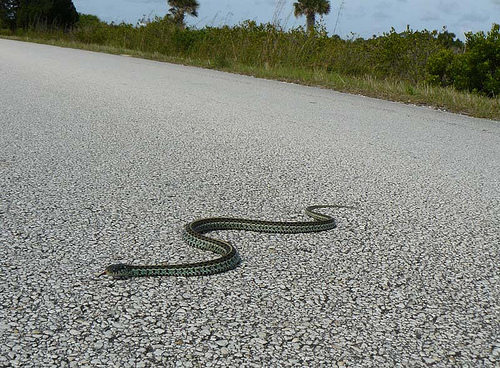
\includegraphics[trim={36mm 10mm 32mm 10mm},clip, width=\sizeP\textwidth]{fig/opticam/images/select/ILSVRC2012_val_00000006.JPEG}&
        \fig[\sizeS]{opticam/images/select/ILSVRC2012_val_00000006JPEG_vgg_GradCAM_vis.png} &
        \fig[\sizeS]{opticam/images/select/ILSVRC2012_val_00000006JPEG_vgg_GradCAMPlusPlus_vis.png} &
        \fig[\sizeS]{opticam/images/select/ILSVRC2012_val_00000006JPEG_vgg_ScoreCAM_vis.png} &
        \fig[\sizeS]{opticam/images/select/ILSVRC2012_val_00000006JPEG_vgg_AblationCAM_vis.png} &
        \fig[\sizeS]{opticam/images/select/ILSVRC2012_val_00000006JPEG_vgg_XGradCAM_vis.png} &
        \fig[\sizeS]{opticam/images/select/ILSVRC2012_val_00000006JPEG_vgg_versionP0_vis.png}  \\
    
        \rotatebox{90}{~Tricycle} &
        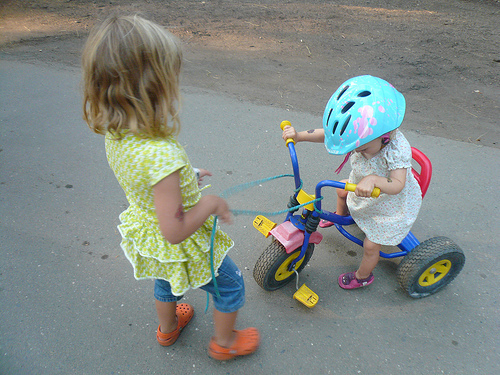
\includegraphics[trim={28mm 10mm 39mm 10mm},clip, width=\sizeP\textwidth]{fig/opticam/images/select/ILSVRC2012_val_00000069.JPEG}&
        \fig[\sizeS]{opticam/images/select/ILSVRC2012_val_00000069JPEG_vgg_GradCAM_vis.png} &
        \fig[\sizeS]{opticam/images/select/ILSVRC2012_val_00000069JPEG_vgg_GradCAMPlusPlus_vis.png} &
        \fig[\sizeS]{opticam/images/select/ILSVRC2012_val_00000069JPEG_vgg_ScoreCAM_vis.png} &
        \fig[\sizeS]{opticam/images/select/ILSVRC2012_val_00000069JPEG_vgg_AblationCAM_vis.png} &
        \fig[\sizeS]{opticam/images/select/ILSVRC2012_val_00000069JPEG_vgg_XGradCAM_vis.png} &
        \fig[\sizeS]{opticam/images/select/ILSVRC2012_val_00000069JPEG_vgg_versionP0_vis.png}  \\

        \rotatebox{90}{~Komondor} &
        \fig[\sizeS]{opticam/images/visual/ILSVRC2012_val_00001113.png}&
        \fig[\sizeS]{opticam/images/visual/Resnet50_GradCAM_ILSVRC2012_val_00001113.png} &
        \fig[\sizeS]{opticam/images/visual/Resnet50_GradCAMPlusPlus_ILSVRC2012_val_00001113.png} &
        \fig[\sizeS]{opticam/images/visual/Resnet50_ScoreCAM_ILSVRC2012_val_00001113.png} &
        \fig[\sizeS]{opticam/images/visual/Resnet50_AblationCAM_ILSVRC2012_val_00001113.png} &
        \fig[\sizeS]{opticam/images/visual/Resnet50_XGradCAM_ILSVRC2012_val_00001113.png} & 
        \fig[\sizeS]{opticam/images/visual/Resnet50_OptCAM_ILSVRC2012_val_00001113.png}  \\
            
        \rotatebox{90}{~Pneumonia} &
        \fig[\sizeS]{opticam/images/medical/chest_VGG16_GradCAM_1_img.png} &
        \fig[\sizeS]{opticam/images/medical/chest_VGG16_GradCAM_1_vis.png} &
        \fig[\sizeS]{opticam/images/medical/chest_VGG16_GradCAMPlusPlus_1_vis.png} &
        \fig[\sizeS]{opticam/images/medical/chest_VGG16_ScoreCAM_1_vis.png} &
        \fig[\sizeS]{opticam/images/medical/chest_VGG16_AblationCAM_1_vis.png} &
        \fig[\sizeS]{opticam/images/medical/chest_VGG16_XGradCAM_1_vis.png} &
        \fig[\sizeS]{opticam/images/medical/chest_VGG16_OptCAM_plain_1_vis.png}  \\
    
    
        \rotatebox{90}{~Pylorus} &
        \fig[\sizeS]{opticam/images/medical/kvasir_Resnet50_GradCAM_3_img.png} &
        \fig[\sizeS]{opticam/images/medical/kvasir_VGG16_GradCAM_3_vis.png} &
        \fig[\sizeS]{opticam/images/medical/kvasir_VGG16_GradCAMPlusPlus_3_vis.png} &
        \fig[\sizeS]{opticam/images/medical/kvasir_VGG16_ScoreCAM_3_vis.png} &
        \fig[\sizeS]{opticam/images/medical/kvasir_VGG16_AblationCAM_3_vis.png} &
        \fig[\sizeS]{opticam/images/medical/kvasir_VGG16_XGradCAM_3_vis.png} &
        \fig[\sizeS]{opticam/images/medical/kvasir_VGG16_OptCAM_plain_3_vis.png}  \\
    
    \end{tabular}
    \caption{\textbf{Saliency maps obtained} by different methods for ImageNet (top two rows), Chest X-ray (row 3) and Kvasir (row 4) with VGG. Ground truth class shown on the left of the input image.}
    \label{fig:vis-in-chest-n-kvasir-resnet}
    % \vspace{-0.4cm}
    \end{figure}
\autoref{fig:vis-in-chest-n-kvasir-resnet} illustrates saliency map examples from ImageNet, Chest 
X-ray and Kvasir datasets. Opti-CAM saliency map is in general more spread out. This better 
highlights full objects, multiple instances or background context, which may be taken into account 
by the model. On Chest X-ray, Opti-CAM and Score-CAM are the only methods that capture the chest, 
while all others focus on image corners. 


%% add more images how?
\section{Quantitaive Evaluation}
\label{sec:oc_quant}
\subsection{Image classification}
%--------------------------------------------------------------------------------------------------
%------------------------------------------------------------------------------
\begin{table}
\centering
\footnotesize
\setlength{\tabcolsep}{4pt}
\renewcommand{\arraystretch}{0.8}
\begin{tabular}{lrrrr|rrrr} \toprule
\mr{2}{\Th{Method}}                                & \mc{4}{\Th{ResNet50}} & \mc{4}{\Th{VGG16}} \\ \cmidrule{2-9}
                                                   & {$\AD\!\downarrow$} & {$\AG\!\uparrow$} & {$\AI\!\uparrow$} & \mc{1}{T} & {$\AD\!\downarrow$} & {$\AG\!\uparrow$} & {$\AI\!\uparrow$} & \mc{1}{T} \\ \midrule
Fake-CAM                &  0.8 &  1.6 & 46.0 &  0.00 &  0.5 &  0.6 & 42.6 &  0.00 \\ \midrule
Grad-CAM                & 12.2 & 17.6 & 44.4 &  0.03 & 14.2 & 14.7 & 40.6 &  0.02 \\
Grad-CAM++              & 12.9 & 16.0 & 42.1 &  0.03 & 17.1 & 10.2 & 33.4 &  0.02 \\
Score-CAM               &  8.6 & 26.6 & 56.7 & 15.22 & 13.5 & 15.6 & 41.7 &  3.11 \\
Ablation-CAM            & 12.5 & 16.4 & 42.8 & 18.26 & 15.5 & 12.6 & 36.9 &  2.98 \\
XGrad-CAM               & 12.2 & 17.6 & 44.4 &  0.03 & 13.8 & 14.8 & 41.2 &  0.02 \\
Layer-CAM               & 15.6 & 15.0 & 38.8 &  0.08 & 48.9 &  3.1 & 13.5 &  0.07 \\
ExPerturbation          & 38.1 &  9.5 & 22.5 & 152.96 & 43.0 &  7.1 & 20.5 & 83.20 \\
\hline
Opti-CAM                & \tb{ 1.5} & \tb{68.8} & \tb{92.8} &  4.15 &  \tb{1.3} & \tb{71.2} & \tb{92.7} & 3.94 \\
\bottomrule
\end{tabular}
\caption{\emph{Classification metrics} on ImageNet validation set, using CNNs. $\AD$/$\AI$: 
average drop/increase \autocite{chattopadhay2018grad}; $\AG$: average gain (ours); 
$\downarrow$ / $\uparrow$: lower / higher is better; 
T: \iavr{Average time (sec) per batch of 8 images. Bold: best, excluding Fake-CAM.}}
\label{tab:imagenet-cnn}
% \vspace{-0.2cm}
\end{table}
%------------------------------------------------------------------------------
% FakeCAM~\citep{poppi2021revisiting}
% Grad-CAM ~\citep{selvaraju2017grad}
% Grad-CAM++~\cite{chattopadhay2018grad}
% ScoreCAM~\citep{wang2020score} 
% AblationCAM~\citep{ramaswamy2020ablation}
% XGrad-CAM~\citep{fu2020axiom} 
% LayerCAM~\citep{jiang2021layercam} 
% ExPerturbation~\citep{fong2019understanding}
%\modify{HiRes-CAM} &\modify{12.2}&\modify{17.6}&\modify{44.4}&\modify{0.03}&\modify{15.8}&\modify{13.2}&\modify{37.8}&\modify{0.02}\\

%--------------------------------------------------------------------------------------------------
\paragraph{CNN}
\autoref{tab:imagenet-cnn} shows ImageNet classification metrics using \Th{VGG16} and \Th{ResNet50}.
 Our Opti-CAM brings impressive performance in terms of average drop ($\AD$) and Average Increase 
 ($\AI$) metrics. That is, not only impressive improvement over baselines, but near-perfect: 
 near-zero $\AD$ and above 90\% $\AI$. Our new metric $\AG$ is lower, around 70\% 
 for Opti-CAM, but this is still several times higher than for all the other methods.

Interestingly, Fake-CAM \autocite{poppi2021revisiting} is the winner in terms of $\AD$ and second 
or third best in $\AI$ after Opti-CAM and Score-CAM, but fails completely $\AG$. This is expected 
and makes Fake-CAM uninteresting as it should be: By only masking one pixel, the classification 
score can hardly drop (0.8\% on ResNet50) and while it increases very often (on 46\% of images), 
the gain is as little as the drop (0.7\%). This makes the pair ($\AD$, $\AG$) sufficient as primary
 metrics and $\AI$ can be thought of as secondary, if important at all.

%In the supplementary material we report \emph{insertion} (I) and \emph{deletion} (D) metrics along with failure cases of Opti-CAM. The latter indicate that our saliency maps are not incorrect as a whole, but capturing more parts of the object, more instances or more background context results in larger or several disconnected salient regions. This does not let the classifier focus on a single discriminative region when pixels are processed sequentially by increasing saliency. Rather, I/D favor smaller and more compact saliency maps.


\autoref{tab:imagenet-cnn} also includes average execution time per image over the 1000-image 
ImageNet subset for all methods. Opti-CAM is slower than gradient-based methods that require 
only one pass through the network, but on par or faster than gradient-free methods. 
Indeed, we use a maximum of 100 iterations with one forward/backward pass per iteration, 
while Score-CAM and Ablation-CAM perform as many forward passes as channels. Hence they are much 
slower on ResNet50 than VGG16. Extremal Perturbation does not depend on the number of channels but 
is very slow by performing a complex optimization in the image space.

%--------------------------------------------------------------------------------------------------
%------------------------------------------------------------------------------
\begin{table}
    \centering
    \footnotesize
    \setlength{\tabcolsep}{4pt}
    \renewcommand{\arraystretch}{0.8}
    \begin{tabular}{lrrrr|rrrr} \toprule
        \mr{2}{\Th{Method}}& \mc{4}{\Th{ViT-B}} & \mc{4}{\Th{DeiT-B}} \\ \cmidrule{2-9}
        & {$\AD\!\downarrow$} & {$\AG\!\uparrow$} & {$\AI\!\uparrow$} & \mc{1}{T} & {$\AD\!\downarrow$} & {$\AG\!\uparrow$} & {$\AI\!\uparrow$} & \mc{1}{T} \\ \midrule
        Fake-CAM            &  0.3 &  0.4 & 48.3 &  0.00 &  0.6 &  0.3 & 44.6 &  0.00 \\ \midrule
        Grad-CAM            & 69.4 &  2.5 & 12.4 &  0.14 & 33.5 &  1.7 & 12.5 &  0.11 \\
        Grad-CAM            & 86.3 &  1.5 &  1.0 &  0.15 & 50.7 &  0.9 &  7.2 &  0.13 \\
        Score-CAM           & 32.0 &  6.2 & 33.0 & 23.69 & 53.6 &  2.2 & 12.2 & 22.47 \\
        XGrad-CAM           & 88.1 &  0.4 &  4.3 &  0.13 & 80.5 &  0.3 &  4.1 &  0.12 \\
        Layer-CAM           & 82.0 &  0.2 &  2.9 &  0.24 & 88.9 &  0.4 &  2.6 & 0.24\\
        ExPerturbation      &28.8&6.2&24.4&133.52&60.9&2.0&8.5&129.12\\
        RawAtt              & 92.6 &  0.2 &  2.8 &  0.02 & 95.3 &  0.0 &  1.8 &  0.02 \\
        Rollout             & 42.1 &  5.6 & 20.9 &  0.02 & 55.2 &  0.8 &  7.9 &  0.02 \\
        TIBAV               & 81.7 &  0.8 &  5.8 &  0.16 & 62.3 &  0.7 &  7.1 &  0.16 \\\midrule
        Opti-CAM            & \tb{ 0.6} &   \tb{18.0} & \tb{90.1} &    16.05 & \tb{ 0.9} & \tb{26.0} & \tb{83.5} &    15.17 \\ \bottomrule
    \end{tabular}
    \caption{}
    %\caption{\emph{Classification metrics} on ImageNet validation set, using transformers. $\AD$/$\AI$: average drop/increase
    %\autocite{chattopadhay2018grad}; $\AG$: average gain (ours); $\downarrow$ / $\uparrow$: lower / higher is better. \iavr{T: Average time (sec) per batch of 8 images. Bold: best, excluding Fake-CAM.}}
    \label{tab:imagenet-trans}
\end{table}
%------------------------------------------------------------------------------
%Fake-CAM~\citep{poppi2021revisiting}    &  0.3 &  0.4 & 48.3 &  0.00 &  0.6 &  0.3 & 44.6 &  0.00 \\ \midrule
%Grad-CAM~\citep{selvaraju2017grad}      & 69.4 &  2.5 & 12.4 &  0.14 & 33.5 &  1.7 & 12.5 &  0.11 \\
%Grad-CAM++~\cite{chattopadhay2018grad}  & 86.3 &  1.5 &  1.0 &  0.15 & 50.7 &  0.9 &  7.2 &  0.13 \\
%Score-CAM~\citep{wang2020score}         & 32.0 &  6.2 & 33.0 & 23.69 & 53.6 &  2.2 & 12.2 & 22.47 \\
%XGrad-CAM~\citep{fu2020axiom}           & 88.1 &  0.4 &  4.3 &  0.13 & 80.5 &  0.3 &  4.1 &  0.12 \\
%Layer-CAM~\citep{jiang2021layercam}     & 82.0 &  0.2 &  2.9 &  0.24 & 88.9 &  0.4 &  2.6 & 0.24\\
%ExPerturbation~\citep{fong2019understanding}&28.8&6.2&24.4&133.52&60.9&2.0&8.5&129.12\\
%RawAtt~\citep{dosovitskiy2020image}     & 92.6 &  0.2 &  2.8 &  0.02 & 95.3 &  0.0 &  1.8 &  0.02 \\
%Rollout~\citep{abnar2020quantifying}    & 42.1 &  5.6 & 20.9 &  0.02 & 55.2 &  0.8 &  7.9 &  0.02 \\
%TIBAV~\cite{chefer2021transformer}      & 81.7 &  0.8 &  5.8 &  0.16 & 62.3 &  0.7 &  7.1 &  0.16 \\
%\modify{HiRes-CAM~\citep{draelos2020use}} &\modify{98.4}&\modify{0.0}&\modify{0.7}&\modify{0.03}&\modify{97.2}&\modify{0.0}&\modify{1.2}&\modify{0.03} \\
%\hline
%Opti-CAM (ours)                         & \tb{ 0.6} &   \tb{18.0} & \tb{90.1} &    16.05 & \tb{ 0.9} & \tb{26.0} & \tb{83.5} &    15.17 \\ \bottomrule
%--------------------------------------------------------------------------------------------------

\paragraph{Transformers}

\autoref{tab:imagenet-trans} shows ImageNet classification metrics using ViT \iavr{and DeiT}. 
Unlike CAM-based methods that rely on a class-specific linear combination of feature maps, 
raw attention \autocite{dosovitskiy2020image} and rollout \autocite{abnar2020quantifying} use the 
attention map of the [CLS] token from the last attention block and from all blocks respectively. 
\iavr{This attention map depends only on the particular image and not on the target class, hence it
 is not really comparable. TIBAV \autocite{chefer2021transformer} uses both instance-specific and 
 class-specific information.

Opti-CAM outperforms all other methods dramatically, reaching near-zero $\AD$ and $\AI$ above 80 or 
90\%. According to our new $\AG$ metric, Opti-CAM still works while all other methods fail, 
but $\AG$ is much more conservative than $\AI$. On ViT-B for example, the classification score 
increases for 90.1\% of the images by masking with Opti-CAM, but the gain is only 18.0\% on average.}

\paragraph{More metrics}
In this section, we show additional metrics including AOPC \autocite{samek2016evaluating}, Max-Sensitivity
 \autocite{yeh2019fidelity} and ADCC \autocite{poppi2021revisiting}.

We use the code and suggested parameters of package 
Quantus\footnote{\url{https://github.com/understandable-machine-intelligence-lab/Quantus}} to measure AOPC 
and MS. In particular, patch size $14$ and number of evaluation regions $10$ for AOPC; lower bound $0.2$ 
and number of samples $10$ for MS.
For ADCC, we use the official 
code\footnote{\url{https://github.com/aimagelab/ADCC?fbclid=IwAR0YK_93lxp4pZQnt34SlA9aeNCLRX8m0u8yTZPxbTXi80qiyhTiqxWaQ7o}}.
We evaluate these metrics on ImageNet validation set using ResNet50 and VGG16. The results are 
reported in \autoref{tab:more-metrics-asked}. Since AOPC shares the same philosophy as I/D, it is 
not a surprise that Opti-CAM has poor performance on AOPC. Opti-CAM achieves the best performance on MS.


\begin{table}[]
\centering
\footnotesize
\setlength{\tabcolsep}{4pt}
\begin{tabular}{lrrr rrr} \toprule
\mr{2}{\Th{Method}} & \mc{3}{\Th{ResNet50}} & \mc{3}{\Th{VGG16}}  \\ \cmidrule{2-7}
                    & {{$AOPC\uparrow$}} & {{$MS\downarrow$}}& {{$ADCC\downarrow$}} & {{$AOPC\uparrow$}} 
                    & {{$MS\downarrow$}}& {{$ADCC\downarrow$}}  \\ \midrule
Grad-CAM            &11.7&1.05&74.3&13.1&1.10&73.7        \\
Grad-CAM++          &11.6&1.04&73.6&11.6&1.09&74.6          \\
Score-CAM           &10.2&1.04&61.0&11.0&1.09&73.9             \\
XGrad-CAM           &11.9&1.05&74.3&13.1&1.10&73.9           \\
Ablation-CAM        &11.1&1.04&71.5&12.5&1.10&75.5          \\
Layer-CAM           &\tb{13.0}&1.22&61.1&\tb{13.3}&1.25&51.7 \\
ExPerturbation      &12.0&1.07&\tb{26.0}&11.2&1.09&\tb{42.8}  \\
\hline
Opti-CAM (ours)     &6.3&\tb{1.03}&65.5&8.9&\tb{1.06}&70.0        \\ \bottomrule

    \end{tabular}
    \caption{\modify{\emph{AOPC/MS/ADCC} scores on ImageNet validation set.}}
    \label{tab:more-metrics-asked}
\end{table}
\section{Object localization}
\label{sec:oc_loc}
\iavr{Localization metrics are used to measure the precision of saliency maps relative to ground truth bounding boxes of the foreground object of interest. These metrics originate from weakly supervised localization (WSOL). However, the objectives of WSOL and explaining the decision of a DNN are not necessarily aligned, since context may play an important role in the decision~\cite{shetty2019not, rao2022towards}.

To investigate the relative importance of the object and its context, we measure classification metrics} when using the bounding box $B$ itself as a saliency map as well as its complement $I \setminus B$, where $I$ is the image. We also evaluate the intersection $B \cap S$ of the saliency map $S$ with the bounding box and with its complement ($S \setminus B$).

As shown in \autoref{tab:localization}, the ground truth region of the object is not the only one responsible for the network decision. For example, the bounding box fails both when used as a saliency map itself and when combined with any saliency map, by harming all classification metrics. Even the complement is more effective than the bounding box itself, either alone or when combined. These findings support the hypothesis that localization metrics based on the ground truth bounding box are not necessarily appropriate for evaluating explanations of network decisions. Classification metrics are clearly more appropriate in this sense.

Nevertheless, we report localization metrics in the supplementary material. In summary, although its saliency maps are more spread out, Opti-CAM outperforms other methods on a number of metrics.

%------------------------------------------------------------------------------
\begin{table}[t]
\footnotesize
\centering
\setlength{\tabcolsep}{4pt}
\renewcommand{\arraystretch}{0.8}
\begin{tabular}{lccc|ccc|ccc} \toprule
\mr{2}{\Th{Method}}                            & \mc{3}{\Th{$\AD\!\downarrow$}} & \mc{3}{\Th{$\AG\!\uparrow$}}& \mc{3}{\Th{$\AI\!\uparrow$}} \\ \cmidrule{2-10}
                                               & {$S$} & {$B \!\cap\! S$} & {$S \!\setminus\! B$} & {$S$} & {$B \!\cap\! S$} & {$S \!\setminus\! B$}& {$S$} & {$B \!\cap\! S$} & {$S \!\setminus\! B$} \\ \midrule
$S \defn B$                                    & 67.2 &   -- &   -- &  2.3 &   -- &   -- &  9.2 &   -- &   -- \\
$S \defn I \setminus B$                        & 44.0 &   -- &   -- &  2.8 &   -- &   -- & 16.3 &   -- &   -- \\ \midrule
Fake-CAM                                       &  0.5 & 67.2 & 44.1 &  0.7 &  2.3 &  2.8 & 42.0 &  9.2 & 18.9 \\ \midrule
Grad-CAM                                       & 15.0 & 72.6 & 52.1 & 15.3 &  1.8 &  6.0 & 40.4 &  8.4 & 19.4 \\
Grad-CAM++                                     & 16.5 & 72.9 & 53.1 & 10.6 &  1.6 &  4.1 & 35.2 &  7.3 & 17.1 \\
Score-CAM                                      & 12.5 & 71.5 & 50.5 & 16.1 &  2.2 &  6.3 & 42.5 &  8.6 & 20.8 \\
Ablation-CAM                                   & 15.1 & 72.8 & 52.1 & 13.5 &  1.7 &  5.6 & 39.9 &  7.8 & 19.0 \\
XGrad-CAM                                      & 14.3 & 72.6 & 51.4 & 15.1 &  1.8 &  6.0 & 42.1 &  8.0 & 20.1 \\
Layer-CAM                                      & 49.2 & 84.2 & 74.4 &  2.7 &  0.4 &  1.2 & 12.7 &  4.4 &  7.3 \\
ExPerturbation                                 & 43.8 & 81.6 & 71.0 &  7.1 &  1.4 &  3.2 & 18.9 &  5.6 & 11.1 \\
\hline
Opti-CAM (ours)                                & \tb{1.4} & \tb{62.5} & \tb{34.8} & \tb{66.3} & \tb{8.7} & \tb{25.8} & \tb{92.5} & \tb{18.6} & \tb{47.1} \\ \bottomrule
\end{tabular}
%\caption{\emph{Bounding box} study. Classification metrics on ImageNet validation set using VGG16. $B$: ground-truth box used by localization metrics; $I$: entire image; $S$: saliency map. $\AD$/$\AI$: average drop/increase~\citep{chattopadhay2018grad}; $\AG$: average gain (ours); $\downarrow$ / $\uparrow$: lower / higher is better; bold: best, excluding Fake-CAM.}
\caption{}
\label{tab:localization}
% \vspace{-0.2cm}
\end{table}
%------------------------------------------------------------------------------

%Fake-CAM~\citep{poppi2021revisiting}
%Grad-CAM~\citep{selvaraju2017grad}             
%Grad-CAM++~\cite{chattopadhay2018grad}
%Score-CAM~\citep{wang2020score}
%Ablation-CAM~\citep{ramaswamy2020ablation}
%XGrad-CAM~\citep{fu2020axiom}                 
%Layer-CAM~\citep{jiang2021layercam}            
%ExPerturbation~\citep{fong2019understanding}   
%--------------------------------------------------------------------------------------------------
\section{Ablation study}
\label{sec:ablation}

We perform an ablation study of different choices of the objective function~\eq{obj} and 
normalization~\eq{norm} of the saliency map. %\redred{More choices of~\eq{obj}, layer $\ell$, number 
%of iterations and learning rates, selector function $g_c$ and initialization of $\vw$ are studied 
%in the supplementary material.}

\paragraph{Normalization function}
For normalization function $n$~\eq{obj}, we investigate three choices:
\begin{align}
	\textrm{range}: \quad & n(A) \defn \textstyle \frac{A-\min A}{\max A-\min A}\label{eq:n-rng}\\
	\textrm{maximum}: \quad & n(A) \defn \textstyle \frac{A}{\max A}\label{eq:n-max}\\
 	\textrm{sigmoid}: \quad & n(a_{ij}) \defn \frac{1}{1+e^{-a_{ij}}}\label{eq:n-sig},
\end{align}
where $a_{ij}$ is element $(i,j)$ of matrix $A$. The default is~\eq{n-rng}, normalizing by the 
range of values in the saliency map, as in Score-CAM~\eq{norm}; while~\eq{n-max} normalizes by the 
maximum value and~\eq{n-sig} by the sigmoid function element-wise.

%--------------------------------------------------------------------------------------------------

\paragraph{Objective function}

We refer to the default definition of $F^c_\ell$~\eq{obj} as \Fdef because it maximizes the logit 
for the masked image.
We also consider an alternative definition of objective function $F^c_\ell$, which encourages the 
masked version to preserve the prediction of original image:
\begin{equation}
	F^c_\ell(\vx; \vu) \defn -\abs{g_c(f(\vx)) - g_c(f(\vx \odot n(\up(S_\ell(\vx; \vu)))))}.
\label{eq:ref}
\end{equation}
This function is named \Fref as it minimizes the difference of logits between the masked and the 
original image.

%--------------------------------------------------------------------------------------------------

\paragraph{Results}

\autoref{tab:ablate} shows classification metrics for the different choices of Opti-CAM, as well as 
comparison to other methods for reference, for the small subset of ImageNet validation set.\\
% \redred{A similar ablation table with localization metrics is available in supplementary material.}

\noindent We observe that the choice of normalization function has little effect overall and Sigmoid 
offers lower performance. Note that the minimum value of saliency maps is often zero or close to 
zero: \emph{Saliency maps are non-negative as convex combinations of non-negative feature maps
~\eq{v-sal}.} In contrast, the choice of loss function has more impact on performance, and we 
observe that \Fdef~\eq{obj} is superior on all cases.

\newcommand{\ob}[1]{\textcolor{brown}{\tb{#1}}}
\newcommand{\ab}[1]{\textcolor{blue}{\tb{#1}}}
\begin{table}[t]
\centering
\footnotesize
\setlength{\tabcolsep}{4pt}
\renewcommand{\arraystretch}{0.8}
\begin{tabular}{lccrrrrr} \toprule
{\Th{Method}} & {$F^c_\ell$} & {$n$} & {$\AD\!\downarrow$}& {$\AG\!\uparrow$} & {$\AI\!\uparrow$}\\ \midrule
Fake-CAM       & & & 0.5  &  0.7 & 42.1 \\
\midrule
Grad-CAM       & & & 15.0 & 15.3 & 40.4 \\
Grad-CAM++     & & & 16.5 & 10.6 & 35.2  \\
Score-CAM      & & & 12.5 & 16.1 & 42.6  \\
Ablation-CAM   & & & 15.1 & 13.5 & 39.9  \\
XGrad-CAM      & & & 14.3 & 15.1 & 42.1  \\
Layer-CAM      & & & 49.2 &  2.7 & 12.7  \\
ExPerturbation & & & 43.8 &  7.1 &  18.9  \\
\midrule
\mr{2}{Opti-CAM} & \Fdef~\eq{obj}  & Range~\eq{n-rng}   & \tb{1.4} & \tb{66.3} & \tb{92.5} \\
	& \Fref~\eq{ref}  & Range~\eq{n-rng}   &     7.1  &     18.5  &     54.9  \\ \midrule
\mr{2}{Opti-CAM} & \Fdef~\eq{obj}  & Max~\eq{n-max}     &     1.6  &     66.2  &     90.3  \\
    & \Fref~\eq{ref}  & Max~\eq{n-max}     &     6.8  &     17.8  &     54.5  \\ \midrule
\mr{2}{Opti-CAM} & \Fdef~\eq{obj}  & Sigmoid~\eq{n-sig} &     5.0  &     18.3  &     57.5  \\
    & \Fref~\eq{ref}  & Sigmoid~\eq{n-sig} &     6.5  &     10.0  &     45.3  \\ \bottomrule
\end{tabular}
\caption{\textbf{Ablation study} using VGG16 on 1000 images of ImageNet validation set. $\AD$/$\AI$: 
average drop/increase \autocite{chattopadhay2018grad}; $\AG$: average gain (ours); $\downarrow$ / 
$\uparrow$: lower / higher is better; bold: best, excluding Fake-CAM.}
\label{tab:ablate}
% \vspace{-0.2cm}
\end{table}
%------------------------------------------------------------------------------

%------------------------------------------------------------------------------
%\pgfplotstableread{fig/eval/plain_ai.dat}{\plotAI}
%\pgfplotstableread{fig/eval/plain_ad.dat}{\plotAD}
%\pgfplotstableread{fig/eval/plain_ag.dat}{\plotAG}
%------------------------------------------------------------------------------

%--------------------------------------------------------------------------------------------------
\section{Discussion}
\label{sec:discuss_opticam}
\noindent Opti-CAM is constructed following the definition of \emph{CAM-based} saliency maps. In 
particular, according to \autoref{eq:sal}, we optimize the variable $w^c_k$ to construct a 
saliency map $S^c_\ell(\mathbf{u})$, maximizing the predicted probability of the explanation 
obtained by performing element-wise multiplication with an input image. \\

\paragraph{Classifier-Centric Explanations} As a consequence of optimizing prediction probability 
of explanation maps, our approach highlights the salient regions in the image. In CNNs, salient 
information is spread across the input image and not often centered within the object of interest; 
these models learn biases within data, and use context to construct a prediction. Furthermore, 
studies have demonstrated instances in fine-grained image classification, where the model learns 
the background of images instead of the object of interest \autocite{petryk2022guiding}. 
Classifier-centric explanations can demonstrate situations where this is the case. Moreover, 
classifier-centric explanations are desired as they do not leave space for human interpretations 
about the inference process of a model, in turn removing one factor of bias towards interpretation.\\

\paragraph{Localization Properties} A direct consequence of generating \emph{classifier-centric 
explanations}, is a trade-off in localization properties. Compared to current 
attribution methods, Opti-CAM fails in this regard. Preliminary studies suggesting the evaluation 
of saliency maps based on these properties, can be traced back to the work by (\cite{shetty2019not}, 
\cite{zhou2018interpreting}, \cite{rao2022towards}). This behavior however is not completely 
undesired. Instead, it highlights that context is important towards prediction of a model; and as 
such localization is an ill-fitted requirement to assess interpretability.\\

\paragraph{Computational Complexity} Opti-CAM generates an optimized saliency map for every image. 
However, in comparison to current high-performing \emph{CAM} attributions, the trade-off of 
complexity and performance favors our approach. In detail, methodologies such as \emph{Ablation-CAM} and 
\emph{Score-CAM} require as many forward passes as the number of channels in the target layer of 
interest. In contrast, our approach requires as much as a hundred optimization steps. 
Additionally, these optimization steps are not as complex as a complete forward pass through the 
network: our optimization objective requires forwarding the product of the optimization variable,
with the feature maps from our target layer until the classifier. As a result, Opti-CAM requires
less memory resources; as well as being faster in running time.\\

\paragraph{Average Gain} Current classification/recognition metrics are not robust and complete,
to differentiate interpretability properties of different approaches. On one hand, this is 
demonstrated in the work of \autocite{poppi2021revisiting}. On the other hand, Average-Gain 
is designed to address this remark. In particular, Average Gain acts as the complement of 
\emph{Average Drop}: we can measure the positive impact that an explanation poses using Average 
Gain. Conversely, \emph{Increase in Confidence} is a metric that on itself does not answer to 
anything in particular: on a real world application we should not care in how many instances the 
explanation map is better than an input image; we ought to focus on the effect an explanation 
has over the classifier.\\
\section{Conclusion}
\label{sec:conclusion}
%--------------------------------------------------------------------------------------------------
% In this work we introduce Opti-CAM, a simple method to visualize saliency maps obtained from 
%different layers of convolutional neural networks, in an effort to make progress in interpreting 
%their predictions.
In this chapter we propose Opti-CAM, a CAM-based methodology to generate saliency maps highlighting 
the most relevant image patches describing a classification according to a classifier. Our approach 
builds upon the definition of CAM attributions to optimize attribution map predicted probabilities.\\

\noindent Opti-CAM combines ideas of different saliency map generation methods, which are masking-based 
and CAM-based. Our method optimizes the saliency map at inference given a single input image. It does 
not require any additional data or training any other network, which would need interpretation too.\\

\noindent While Opti-CAM crafts a saliency map in the image space, it does not need any 
regularization. This is because the saliency map is expressed as a convex combination of feature 
maps, and we only optimize one vector over the feature dimensions. The underlying assumption is 
that of all CAM-based methods: feature maps contain activations at all regions that are of 
interest for the classes that are present. Opti-CAM is more expensive than non-iterative 
gradient-based methods but as fast or faster than gradient-free methods that require as many 
forward passes as channels.\\

\noindent Opti-CAM brings impressive performance improvement over the state of the 
art according to the most important classification metrics on several datasets. The saliency maps 
are more spread out compared with those of the competition, attending to larger parts of the object, 
multiple instances and background context, which may be helpful in classification.\\

%By contrast, the same property may harm localization metrics in case the saliency map extends beyond the ground-truth bounding box of the object of interest. Indeed, our results are mixed in terms of localization metrics.

\noindent Our new classification metric $\AG$ aims to be paired $\AD$ as a replacement of 
$\AI$ and resolves a long-standing problem in evaluating attribution methods, without further 
increasing the number of metrics. We provide strong evidence supporting that the use of 
ground-truth object bounding boxes for localization is not necessarily optimal in evaluating 
the quality of a saliency map, because the primary objective is to explain how a classifier works.
% and not to localize objects in a weakly-supervised setting.


